%'pdflatex "Fourier Series and Fourier Transform.tex"' to create pdf
\documentclass[12pt]{article}
\usepackage{amsmath}
\usepackage{amsfonts, amssymb}   %amsfonts is for xER
\usepackage{graphicx}       % for inserting pictures
\usepackage{tikz}           % for creating graphs and diagrams
\graphicspath{ {./img/} }   % source of pictures (path relative to the main .tex file) 
\usepackage{titlesec}               % for automatic \newpage after every section
\newcommand{\sectionbreak}{\clearpage}      % automatic \newpage after every section
\counterwithin*{equation}{section}      % resets the equation numbering system for every section
\usepackage{color}
\usepackage{hyperref}       % for clickable table of contents and links
\hypersetup{
    colorlinks,
    citecolor=black,
    filecolor=black,
    linkcolor=black,
    urlcolor=black
}


\title{Fourier Transform and Laplace Transform Notes} 
\author{Me}



\begin{document} 
\maketitle 
\tableofcontents 



%------------------------------------------------------------------------------------------------------------
%------------------------------------------------------------------------------------------------------------
%----------------------------------------------- Introduction -----------------------------------------------
%------------------------------------------------------------------------------------------------------------
%------------------------------------------------------------------------------------------------------------
%\addcontentsline{toc}{section}{Introduction}
\section{Introduction}
\indent Similar to the concept of the Taylor Series, 
all functions can be written as sum of cosine and sine 
functions with different weightings and frequencies. 

\vspace{25pt}
\begin{figure}[h]
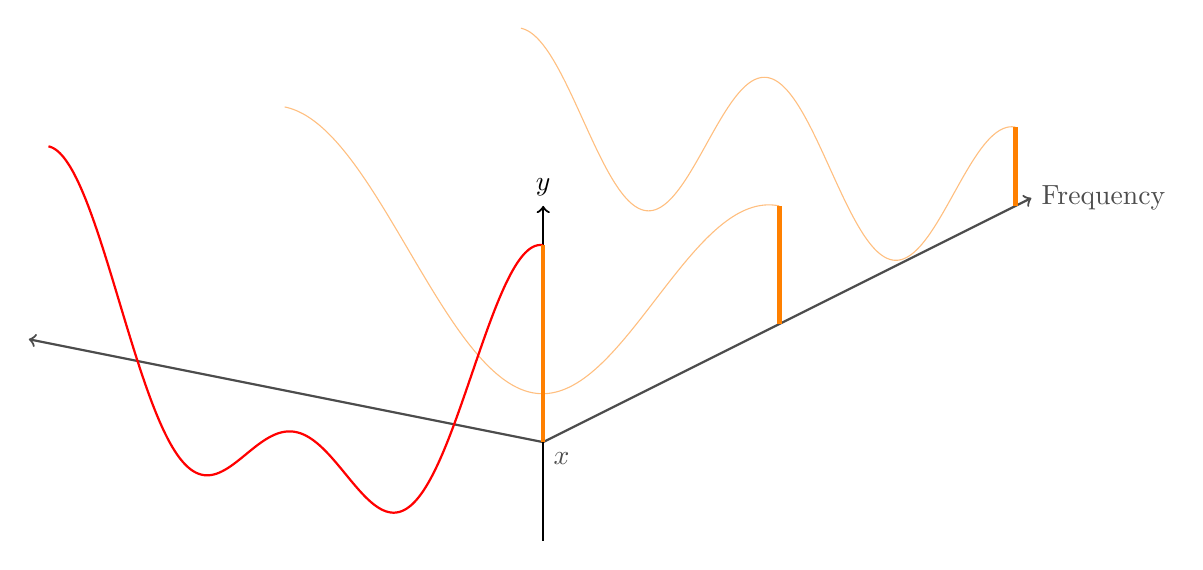
\begin{tikzpicture}[x={(1cm,0.5cm)},z={(0cm,0.5cm)},y={(1cm,-0.2cm)}]
    \draw[->,thick,black!70] (0,0,0) -- (6.2,0,0) node[right] {Frequency}; % 频率轴
    \draw[<-,thick,black!70] (0,-2*pi-0.25,0) -- (0,0,0) node[below right] {$x$}; % 时间轴
    \draw[->,thick] (0,0,-2.5) -- (0,0,6) node[above] {$y$}; 

    \draw [orange!50, domain=-2*pi:0,samples=300,smooth] 
        plot (3,\x, {3*cos(180*\x/pi) });
    \draw[orange, ultra thick] (3,0,0) -- (3,0,3);

    \draw [orange!50, domain=-2*pi:0,samples=300,smooth] 
        plot (6,\x, {2*cos(360*\x/pi) });
    \draw[orange, ultra thick] (6,0,0) -- (6,0,2);
    
    \draw [red, thick, domain=-2*pi:0,samples=300,smooth] 
        plot (0,\x, {3*cos(180*\x/pi) + 2*cos(360*\x/pi});
    \draw[orange, ultra thick] (0,0,0) -- (0,0,5);
    
\end{tikzpicture}
\caption{an example of periodic function summation}
\label{fig:intro_example}
\end{figure}
\vspace{25pt}

\indent Figure \ref{fig:intro_example} is a periodic function, and it can be broken down into 
the sum of two cosine functions $f(x)=3\cos(x)+2\cos(2x)$.  %\newpage

This concept of transformation is the fundamental of Fourier Transform as the name suggests,
and has great application in many field of study, for example, signal processing. 
The function of time would be converted into the functions of frequency. 
It used to be difficult to isolate or manipulate some certain frequencies with the function of time, 
but we can convert/transform it into the functions of frequency, then do whatever needs to be done. 
It can be again transformed back into the function of time when needed.












%------------------------------------------------------------------------------------------------------------
%------------------------------------------------------------------------------------------------------------
%---------------------------------------------- Fourier Series ----------------------------------------------
%------------------------------------------------------------------------------------------------------------
%------------------------------------------------------------------------------------------------------------
%\addcontentsline{toc}{section}{Fourier Series}
\section{Fourier Series}
\indent The Fourier Series expresses periodic functions as 
sums of weighted cosine and sine functions of different frequencies, 
where the frequencies are integer multiples of the base freqeuncy (frequency of the periodic function).
Every non constant term in the Fourier Series are defined as 
a coefficient multiplied by a cosine or sine function of a frequency.

%\addcontentsline{toc}{subsection}{Evaluation of Constants and Coefficients}
\subsection{Evaluation of Constants and Coefficients}
\indent However, most of the time, we only have some information about the function, 
and we are required to construct the Fourier Series for the function. 
The major challenge is to find out the coefficients for every frequencies in order to do so.

\indent The general formula of the Trigonometric Fourier Series can be written as
\begin{equation}
    f(t) = a_0 + \sum_{n=1}^{\infty}a_n\cos(\frac{2n\pi t}{T}) + \sum_{n=1}^{\infty}b_n\sin(\frac{2n\pi t}{T})
    \label{equ:trig_fourier_series_expansion}
\end{equation}
, where $T$ is the period of $f(t)$, and $n\in\mathbb{Z}$.

\indent For a periodic function $f(t)$ with a period of $T$, 
we noticed that taking the definite integral of $f(t)$ from the start of a cycle to the end of the cycle
then divided by the period (length of a cycle) gives the average value of $f(t)$. 
$$  
    \frac{1}{T}     \int_{T}f(t)\mathrm{d}t
    = \frac{1}{T}   \int_{T}a_0\mathrm{d}t
    + \frac{1}{T}   \sum_{n=1}^{\infty}   a_n   \int_{T}\cos(\frac{2n\pi t}{T})\mathrm{d}t
    + \frac{1}{T}   \sum_{n=1}^{\infty}   b_n \int_{T}\sin(\frac{2n\pi t}{T})\mathrm{d}t
$$
Evaluate the definite integrals on the right side of the equation:
$$      \int_{T} a_0 \mathrm{d}t    =   a_0  T                  $$
$$      \int_{T}\cos(\frac{2n\pi t}{T})\mathrm{d}t  = 0         $$
$$      \int_{T}\sin(\frac{2n\pi t}{T})\mathrm{d}t  = 0         $$

We sub in the results into the equation and simplify it to get:
\begin{equation}
    a_0  =  \frac{1}{T} \int_{T} f(t) \mathrm{d}t
    \label{equ:fourier_series_a0_term}
\end{equation}


\indent Using this method, we get the average of the periodic function, 
or in other words the term we evaluated the term $a_0$. However, 
we still have to find a way to calculate the rest of the coefficients.
Before doing so, we have to know some knowledge about definite integrals of cosine and sine functions. 
For any constant $a_0$ and integers $m$ and $n$ where $m\not=n$:
$$      \int_{2\pi} a_0\cos(mx) \mathrm{d}x    =   0            $$
$$      \int_{2\pi} a_0\sin(mx) \mathrm{d}x    =   0            $$
$$      \int_{2\pi} \cos(mx)\sin(nx) \mathrm{d}x    =   0       $$
$$      \int_{2\pi} \cos(mx)\cos(nx) \mathrm{d}x    =   0       $$
$$      \int_{2\pi} \sin(mx)\sin(nx) \mathrm{d}x    =   0       $$
$$      \int_{2\pi} \cos(mx)\sin(mx) \mathrm{d}x    =   0       $$
$$      \int_{2\pi} \cos^2(mx) \mathrm{d}x    =   \pi           $$
$$      \int_{2\pi} \sin^2(mx) \mathrm{d}x    =   \pi           $$
\indent From the above equations, we know that multiplying a cosine or sine function by 
another cosine or sine function of a different frequency before taking the definite integral 
does not have a influence on the result. The exception is that when it is multiplied by itself, 
the result changes from $0$ to $\pi$. This is useful, 
we can multiply $f(t)$ by the desired cosine or sine function that contains the desired frequency 
to get the corresponding coefficient of the term.
\begin{equation}
    a_n =   \frac{2}{T} \int_{T} f(t)\cos(\frac{2n\pi t}{T}) \mathrm{d}t
    \label{equ:trig_fourier_series_cosine_coeff}
\end{equation}
\begin{equation}
    b_n =   \frac{2}{T} \int_{T} f(t)\sin(\frac{2n\pi t}{T}) \mathrm{d}t
    \label{equ:trig_fourier_series_sine_coeff}
\end{equation}



%\addcontentsline{toc}{subsection}{Fourier Spectrum}
\subsection{Fourier Spectrum}
Since a periodic function can be expressed as a fourier series, 
we can use spectrums to defined a fourier series where the x-value would be the frequency of the term instead of time,
and the y-value could be the corresponding amplitude/coefficient of the term 
or the corresponding phase shift of the term. 





%\addcontentsline{toc}{subsubsection}{Single_Sided Spectra}
\subsubsection{Single-Sided Spectra}
In equation ({\ref{equ:trig_fourier_series_expansion}}), there are four parameters we have to figure out, 
which is a lot of calculation. We can reduce them, since the sum of cosine and sine function of the same frequency 
can be expressed in one single term of cosine or sine function using the Sum-to-Product Identities. 
This would add an extra parameter, phase shift into the equation, 
however, it removes the amplitude of cosine or sine function, and the corresponding frequency. 
After combining the cosine terms and the sine terms into only cosine or sine terms, 
every term in the trigonometric form of a periodic function can be described using 
three parameters: amplitude, frequency and phase shift. 
Let $\omega_0$ be the base frequency, and $\omega_0=\frac{2\pi}{T}$.
This can be proved. From ({\ref{equ:trig_fourier_series_expansion}}), 
we can combine the cosine and sine functions that has the same frequency together into one single term, 
because a cosine function added to a sine function is a shifted, compressed or stretched cosine or sine function.
Let $C_0 = D_0 = a_0$ we obtain the compacted form of the fourier series:

\begin{equation}
    f(t) =      C_0     +   \sum_{n=1}^{\infty} C_n \cdot \cos(n\omega_0t+\phi_n)
    \label{equ:fourier_spectrum_cosine}
\end{equation}
\begin{equation}
    f(t) =      D_0     +   \sum_{n=1}^{\infty} D_n \cdot \sin(n\omega_0t+\theta_n)
    \label{equ:fourier_spectrum_sine}
\end{equation}

$n\omega_0$ in this equation is the frequency of each term, 
$C_n$ and $D_n$ are the amplitudes of the corresponding frequency,
and $\phi_n$ is the corresponding phase shift. Both (\ref{equ:fourier_spectrum_cosine}) 
and (\ref{equ:fourier_spectrum_sine}) would work, 
but (\ref{equ:fourier_spectrum_cosine}) is peferred most of the times. 
We would use (\ref{equ:fourier_spectrum_cosine}) in this subsection.

This concept can be proved algebrically. 
$$\begin{aligned}
f(t) &= C_0  +  \sum_{n=1}^{\infty} C_n \cdot \cos(n\omega_0t+\phi_n)   \\
&= C_0  +  \sum_{n=1}^{\infty} C_n \left[ \cos(n\omega_0t)\cos(\phi_n) - \sin(n\omega_0t)\sin(\phi_n) \right]   \\
&= C_0  +  \sum_{n=1}^{\infty} C_n \cos(n\omega_0t)\cos(\phi_n) - \sum_{n=1}^{\infty} C_n \sin(n\omega_0t)\sin(\phi_n)
\end{aligned}$$

Compare the coefficients of the above equation with (\ref{equ:trig_fourier_series_expansion}), we get:
\begin{equation}
    \begin{cases}
        a_0     =       C_0                 \\
        a_n     =       C_n\cos(\phi_n)     \\
        b_n     =       -C_n\sin(\phi_n)
    \end{cases}
    \label{equ:an_bn_with_Cn_relationship}
\end{equation}

Compute $a_n^2 + b_n^2$ using ({\ref{equ:an_bn_with_Cn_relationship}}) would gives the first equation below, 
and divide $b_n$ by $a_n$ gives the second equation below, we obtain:
\begin{equation} \begin{cases}
    C_0 = a_0       \\
    C_n^2     =       a_n^2     +       b_n^2       \\
    \tan(\phi_n)   =    -\frac{b_n}{a_n}
    \label{equ:Cn_an_bn_relationship}
\end{cases} \end{equation}

Since we can convert any $a_n\cos(n\omega_0t)+b_n\sin(n\omega_0t)$ into $C_n\cos(n\omega_0t+\phi_n)$ 
using ({\ref{equ:Cn_an_bn_relationship}}), therefore, this concept holds for cosine function. 
Similar conclusions can be made using the same proccess with sine function:
\begin{equation} \begin{cases}
    D_0 = a_0       \\
    D_n^2     =       a_n^2     +       b_n^2       \\
    \tan(\theta_n)   =    \frac{a_n}{b_n}
    \label{equ:Dn_an_bn_relationship}
\end{cases} \end{equation}

Extending this concept, for real numbers of $k_n$, $\theta$ and $\phi$: 
$$\begin{aligned}
       & k_1\cos(x) + k_2\sin(x) + k_3\cos(x+\phi) + k_4\sin(x+\theta) \\
    =& k_1\cos(x) + k_2\sin(x) + k_3\cos(\phi)\cos(x) - k_3\sin(\phi)\sin(x) + \\
    &k_4\cos(\phi)\sin(x) + k_4\sin(\phi)\cos(x)  \\
    =& \left[k_1 + k_3\cos(\phi) + k_4\sin(\phi)\right] \cos(x) + \left[k_2 - k_3\sin(\phi) + k_4\cos(\phi)\right]\sin(x)   \\
\end{aligned}$$

\indent Then sub values into ({\ref{equ:Cn_an_bn_relationship}}) and ({\ref{equ:Dn_an_bn_relationship}}) 
gives the amplitude and phase shift.

\indent After we figure out all of the frequency and their corresponding amplitudes and phase shift, 
we can create two graphs that describes the fourier series: the amplitude spectrum and the phase spectrum.
Nevertheless, the spectrums are not continous due to the frequecies of 
the terms in the fourier series not being continous. The graphs are only defined at inputs of all whole numbers 
(zero and all positive integers). Because the fourier series only includes positive frequencies.
 

\textbf{Example:}

The following is an example of the graphs of 
$f(t) = 4\cos(10\pi t+\frac{\pi}{4}) - 6\cos(20\pi t+\frac{\pi}{6}) + 2\sin(40\pi t+\frac{\pi}{3})$.
$$f(t)= 4\cos(10\pi t+\frac{\pi}{4}) + 6\cos(20\pi t+\frac{7}{6}\pi) + 2\cos(40\pi t-\frac{\pi}{6})$$
\indent In this example, the base frequency, $\omega_0$ is $10\pi$.
From the fourier series expansion above, we can get the two spectrums:\newline
\begin{figure}[!h]
    \begin{minipage}[c]{0.47\linewidth}
        \centering
        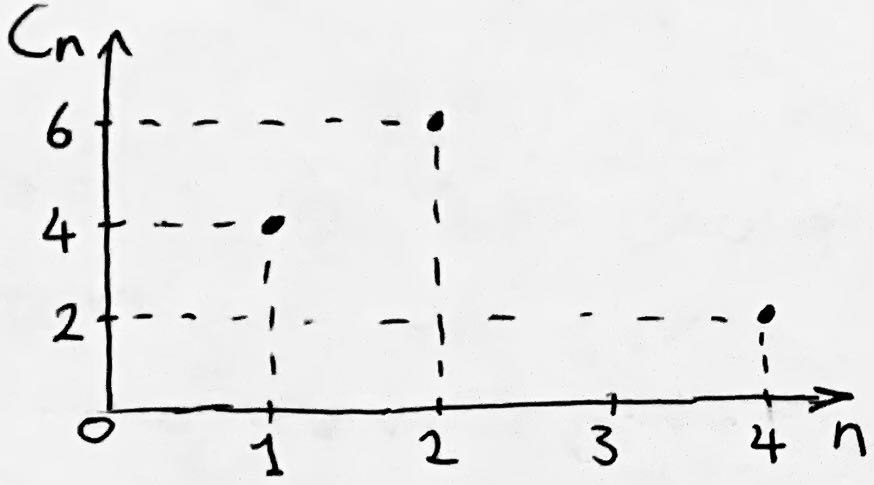
\includegraphics[width=1\linewidth]{fourier_series_single_side_spectrum_example1}
        \caption{the amplitude spectrum}
        \label{fig:fourier_series_single_side_spectrum_example1}
    \end{minipage}\hfill
    \begin{minipage}[c]{0.47\linewidth}
        \centering
        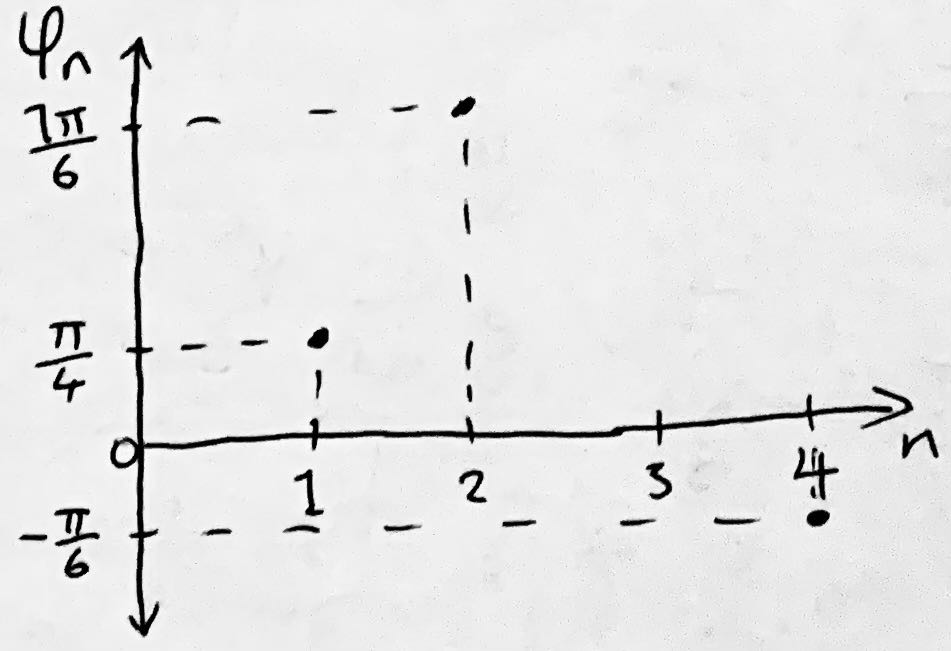
\includegraphics[width=1\linewidth]{fourier_series_single_side_spectrum_example2}
        \caption{the phase spectrum}
        \label{fig:fourier_series_single_side_spectrum_example2}
    \end{minipage}
\end{figure}


%\addcontentsline{toc}{subsubsection}{Two-Sided Spectra}
\subsubsection{Two-Sided Spectra}
From Euler's formula $e^{\mathrm{i}x}=\cos{x}+\mathrm{i}\sin{x}$, we can deduce to get:
\begin{equation}
    \begin{cases}
        \cos(n\omega_0t) = \frac{1}{2}\left[e^{\mathrm{i}n\omega_0t}+e^{-\mathrm{i}n\omega_0t}\right]   \\
        \sin(n\omega_0t) = -\frac{\mathrm{i}}{2}\left[e^{\mathrm{i}n\omega_0t}-e^{-\mathrm{i}n\omega_0t}\right]
    \end{cases}
    \label{equ:cosine_and_sine_in_exponential_form}
\end{equation}
Substitute ({\ref{equ:cosine_and_sine_in_exponential_form}}) into ({\ref{equ:trig_fourier_series_expansion}}), 
we obtain:

$$\begin{aligned} f(t) =& a_0 + 
\sum_{n=1}^{\infty}\frac{a_n}{2}\left[e^{\mathrm{i}n\omega_0t}+e^{-\mathrm{i}n\omega_0t}\right]
+ \sum_{n=1}^{\infty}\frac{b_n}{2\mathrm{i}}\left[e^{\mathrm{i}n\omega_0t}-e^{-\mathrm{i}n\omega_0t}\right] \\
=& a_0 + \sum_{n=1}^{\infty}\left[ \frac{a_n-\mathrm{i}b_n}{2}e^{\mathrm{i}n\omega_0t} 
+ \frac{a_n+\mathrm{i}b_n}{2}e^{-\mathrm{i}n\omega_0t}\right]   \\
=& a_0 + \sum_{n=1}^{\infty}\left[ \frac{a_n-\mathrm{i}b_n}{2}e^{\mathrm{i}n\omega_0t} \right]
+ \sum_{n=-\infty}^{-1}\left[\frac{a_{-n}+\mathrm{i}b_{-n}}{2}e^{\mathrm{i}n\omega_0t}\right]
\end{aligned}$$

By Substituting $-n$ into (\ref{equ:trig_fourier_series_cosine_coeff}) and 
(\ref{equ:trig_fourier_series_sine_coeff}), we obtain:
\begin{equation}\begin{cases}
    a_n = a_{-n}    \\
    b_n = -b_{-n}
\end{cases}
\label{equ:coeff_of_negative_n_relationship}
\end{equation}

Let $F_n=\frac{a_n-\mathrm{i}b_n}{2}$, and $F_0=a_0$:

$$\begin{aligned} f(t) =& a_0 + 
    \sum_{n=1}^{\infty}\left[ \frac{a_n-\mathrm{i}b_n}{2}e^{\mathrm{i}n\omega_0t} \right]
    + \sum_{n=-\infty}^{-1}\left[\frac{a_n-\mathrm{i}b_n}{2}e^{\mathrm{i}n\omega_0t}\right] \\
    =& F_0e^{0\mathrm{i}n\omega_0t} + 
    \sum_{n=1}^{\infty}F_ne^{\mathrm{i}n\omega_0t}
    + \sum_{n=-\infty}^{-1}F_ne^{\mathrm{i}n\omega_0t}
\end{aligned}$$

Continue simplifying this equation, we deduced the exponential fourier series:
\begin{equation}
    f(t) = \sum_{n=-\infty}^{\infty}F_ne^{\mathrm{i}n\omega_0t}
\end{equation}

Expand $F_n$ with (\ref{equ:trig_fourier_series_cosine_coeff}) and (\ref{equ:trig_fourier_series_sine_coeff}):
$$\begin{aligned} 
    F_n 
    =& \frac{a_n-\mathrm{i}b_n}{2}    \\
    =& \frac{1}{2}\cdot\frac{2}{T} \int_{T} f(t)\cos(n\omega_0t) \mathrm{d}t   
        - \frac{\mathrm{i}}{2}\cdot\frac{2}{T} \int_{T} f(t)\sin(n\omega_0t) \mathrm{d}t
\end{aligned}$$
\indent Apply Euler's formula:
\begin{equation}
    F_n = \frac{1}{T}\int_{T} f(t)e^{-\mathrm{i}n\omega_0t} \mathrm{d}t
    \label{equ:fourier_series_exponent_coeff}
\end{equation}

\indent We had removed another parameter from the equation, combining the amplitudes and phase shifts informations 
into a single complex number, $F_n$. The magnitude of $F_n$ describes amplitude, 
and the argument of it describes phase shifts.
Since $F_n = \left|F_n\right|e^{\mathrm{i}\phi_n}$ is a complex number, 
we can calculate the magnitude and argument:

$$\begin{cases}
    \left|F_0\right| = C_0 = D_0  \\
    \left|F_n\right| = \frac{1}{2}\sqrt{a_n^2+b_n^2} = \frac{1}{2}C_n = \frac{1}{2}D_n , n > 0   \\
    \tan(\phi_n) = -\frac{b_n}{a_n} = \tan(\phi_n) = -\cot(\theta_n) , n > 0
\end{cases}$$

\indent Since our fourier series included negative values, we can sub in ({\ref{equ:coeff_of_negative_n_relationship}}) 
into the above equation, this suggests that the amplitude, $\left|F_n\right|$ is an even function of $n$, 
while $\phi_n$ is an odd function of $n$. 

$$\begin{cases}
    \left|F_n\right| = \left|F_{-n}\right| \\
    \phi_n = -\phi_{-n}
\end{cases}$$


\noindent\textbf{Example:}

$$f(t) = 4\cos(10\pi t+\frac{\pi}{4}) - 6\cos(20\pi t+\frac{\pi}{6}) + 2\sin(40\pi t+\frac{\pi}{3})$$
\indent Convert the example from the preceeding subsubsection using ({\ref{equ:cosine_and_sine_in_exponential_form}}):

$$\begin{aligned}
    f(t) 
    =& 4\cos(10\pi t+\frac{\pi}{4}) + 6\cos(20\pi t+\frac{7}{6}\pi) + 2\cos(40\pi t-\frac{\pi}{6})  \\
    =& 2e^{\mathrm{i}\pi(10t+\frac{1}{4})} + 3e^{\mathrm{i}\pi(20t+\frac{7}{6})} + e^{\mathrm{i}\pi(40t-\frac{1}{6})} \\
    &+ 2e^{-\mathrm{i}\pi(10t+\frac{1}{4})} + 3e^{-\mathrm{i}\pi(20t+\frac{7}{6})} + e^{-\mathrm{i}\pi(40t-\frac{1}{6})}
\end{aligned}$$


\indent This also works if $f(t)$ is the sum of sine functions. With the same example, 
since $\cos(x)=\sin(x-\frac{\pi}{2})$, 
we can easily convert all of the cosine terms into sine to use the same example. 
Simply by replacing $-\mathrm{i}$ with 
$e^{\frac{\mathrm{i}\pi}{2}}$ would give the exact same result.

$$\begin{aligned}
    f(t) 
    =& 4\sin(10\pi t+\frac{3\pi}{4}) + 6\sin(20\pi t+\frac{5}{3}\pi) + 2\sin(40\pi t+\frac{\pi}{3}) \\
    =& \mathrm{i}2(e^{-\mathrm{i}\pi(10t+\frac{3}{4})} - e^{\mathrm{i}\pi(10t+\frac{3}{4})}) +
    \mathrm{i}3(e^{-\mathrm{i}\pi(10t+\frac{5}{3})} - e^{\mathrm{i}\pi(20t+\frac{5}{3})})       \\
    &+\mathrm{i}(e^{-\mathrm{i}\pi(40t+\frac{1}{3})} - e^{\mathrm{i}\pi(40t+\frac{1}{3})})       \\
    =& 2(e^{\mathrm{i}\pi(10t+\frac{1}{4})} + e^{-\mathrm{i}\pi(10t+\frac{1}{4})} )
    + 3(e^{\mathrm{i}\pi(20t+\frac{7}{6})} + e^{-\mathrm{i}\pi(20t+\frac{7}{6})})               \\
    &+ e^{\mathrm{i}\pi(40t-\frac{1}{6})} + e^{-\mathrm{i}\pi(40t-\frac{1}{6})}
\end{aligned}$$

\begin{figure}[h!]
    \begin{minipage}[c]{0.47\linewidth}
        \centering
        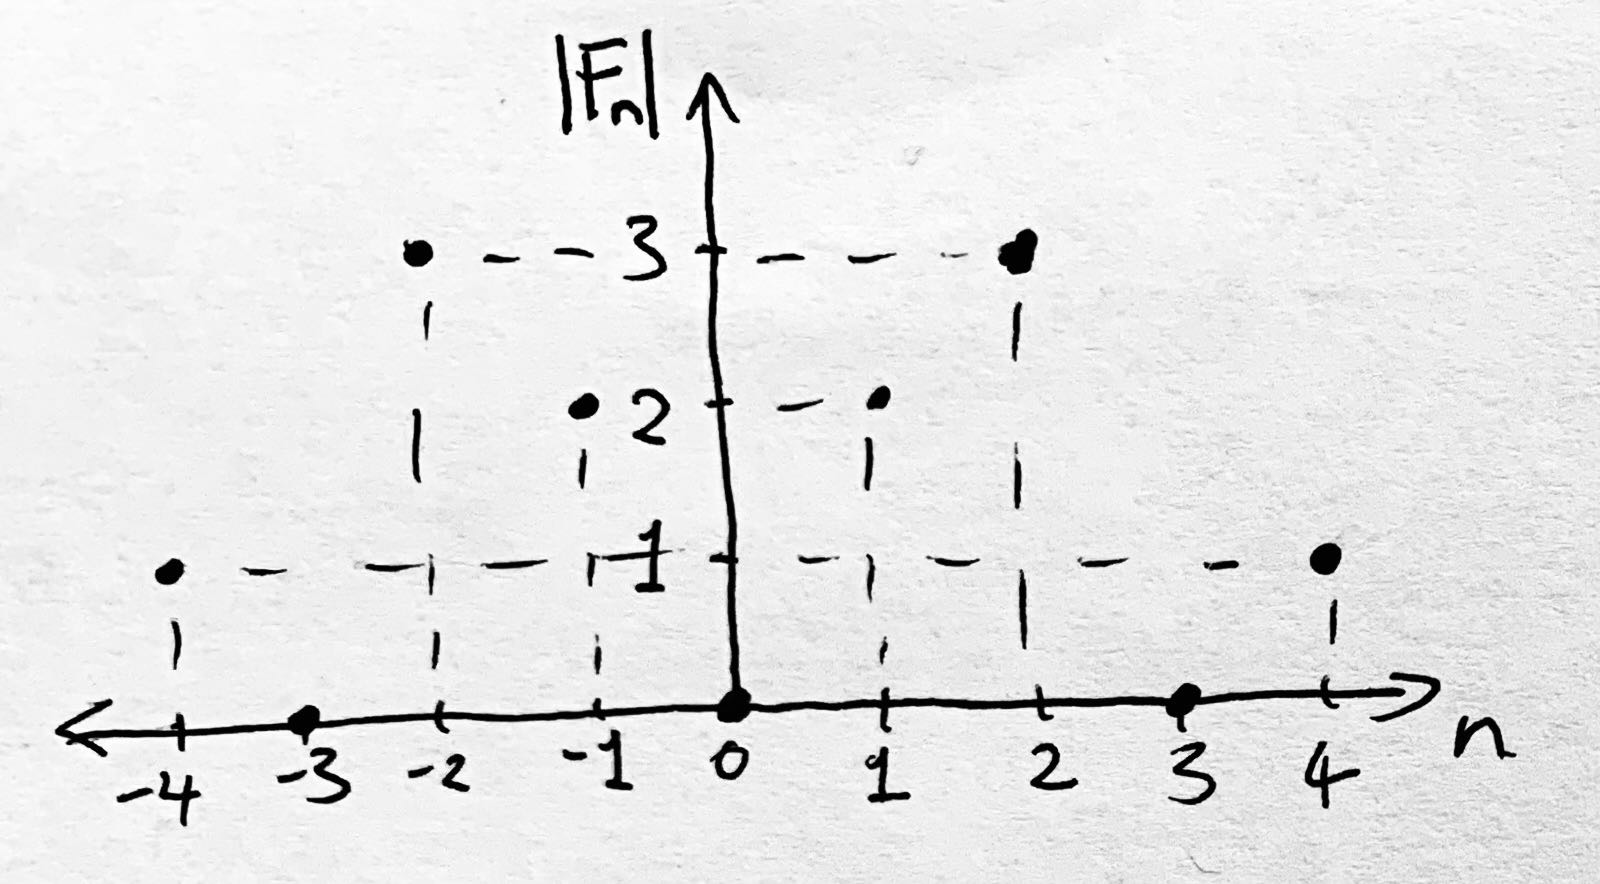
\includegraphics[width=1\linewidth]{fourier_series_two_side_spectrum_example1}
        \caption{the amplitude spectrum}
        \label{fig:fourier_series_two_side_spectrum_example1}
    \end{minipage}\hfill
    \begin{minipage}[c]{0.47\linewidth}
        \centering
        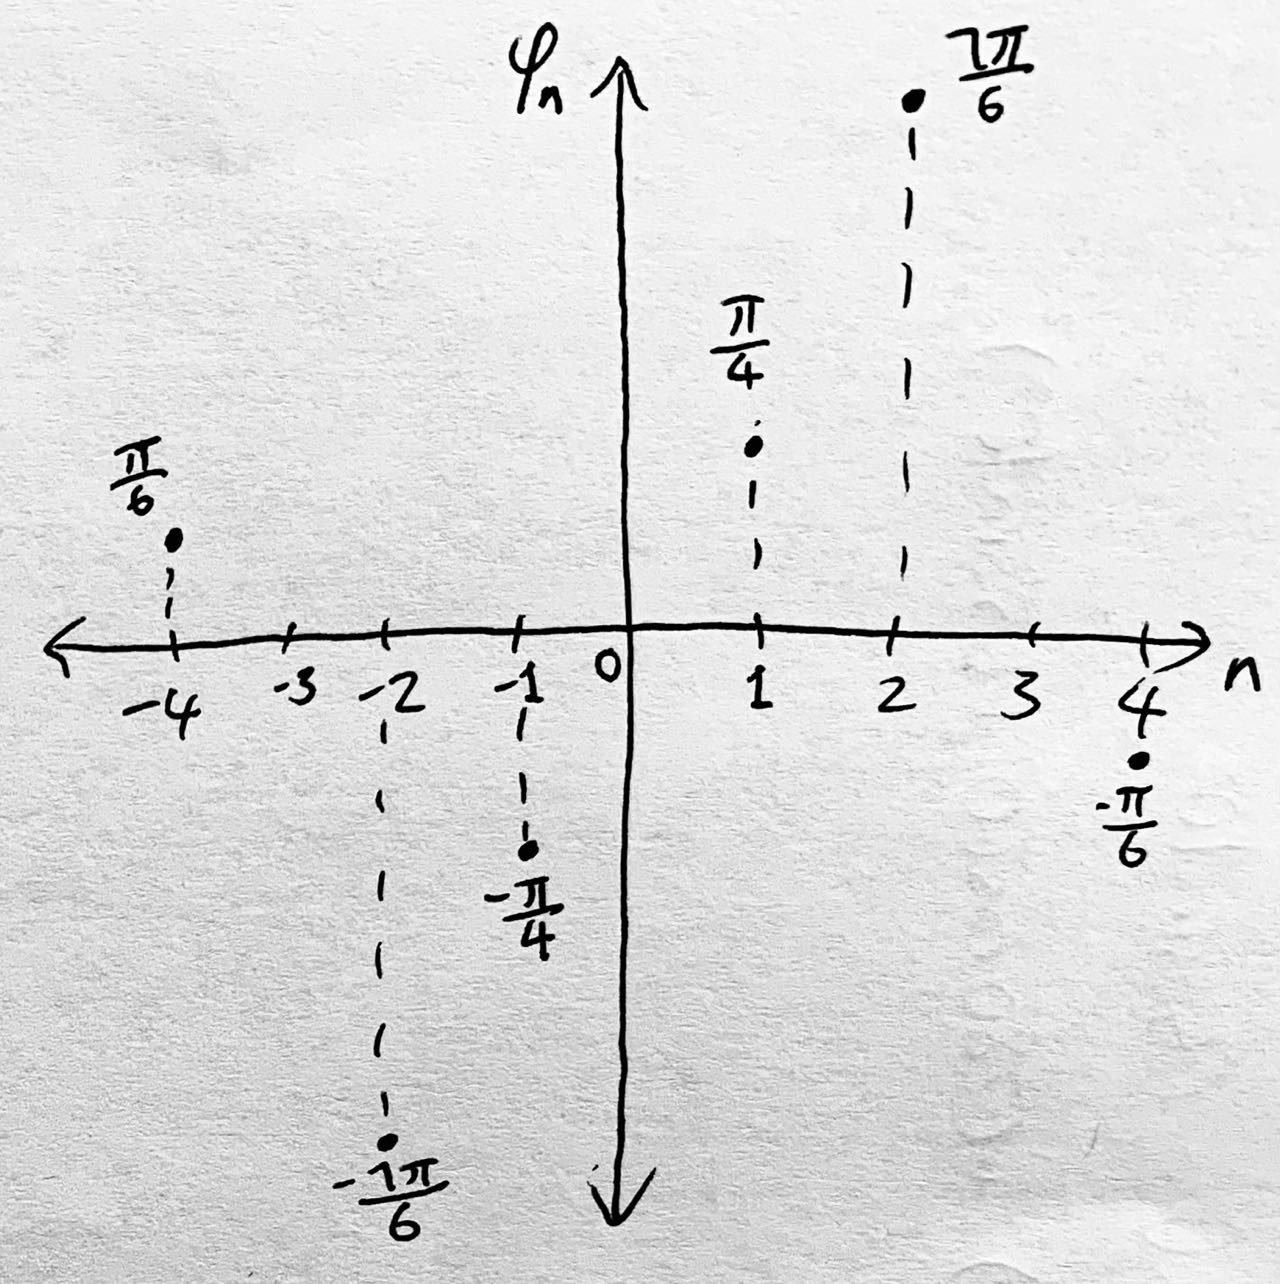
\includegraphics[width=1\linewidth]{fourier_series_two_side_spectrum_example2}
        \caption{the phase spectrum}
        \label{fig:fourier_series_two_side_spectrum_example2}
    \end{minipage}
\end{figure}

\indent Comparing these two graphs with the single-sided spectra, 
it is obvious that they look nearly identical for $n \ge 0$.











%------------------------------------------------------------------------------------------------------------
%------------------------------------------------------------------------------------------------------------
%----------------------------------- Continous Time Fourier Transform (Fourier Integral) -----------------------------------
%------------------------------------------------------------------------------------------------------------
%------------------------------------------------------------------------------------------------------------
%\addcontentsline{toc}{section}{Fourier Transform}
\section{Fourier Transform (Fourier Integral)}
For continous periodic functions, we had showed the transform by using the fourier series, 
we are able to describe the continuous periodic function using amplitude and phase shift instead of time. 
Not only that, the proccess of convertion was also showed. 

Nevertheless, the fourier series can only deal with periodic functions and 
it cannot pick out amplitude and phase shift informations of continous frequencies. 
This is the problem that fourier transform solves.
The fourier integral solves both problems by setting the cycle to $-\infty$ to $\infty$, 
and expand the definition of $n$ to the real number set. 
The entire function becomes one cycle, resulting in the base frequency, 
$\omega_0$ to approach $0$. Due to the fact that $\frac{1}{T}=\frac{\omega_0}{2\pi}$, 
and $\omega_0$ equals to the difference between the two nearby freqeuncy($n\omega_0$ and $(n+1)\omega_0$) 
in the fourier series. 

The equation for the fourier series
$$
    f(t) 
    = \sum_{n=-\infty}^{\infty} \left[ e^{\mathrm{i}n\omega_0t} \cdot
    \frac{\omega_0}{2\pi}\int^{T} f(t)e^{-\mathrm{i}n\omega_0t} \mathrm{d}t\right]
$$
becomes:
$$\begin{aligned}
    f(t) 
    &= \lim_{\omega_0 \to 0} \sum_{n=-\infty}^{\infty} \left[ e^{\mathrm{i}n\omega_0 t} \cdot
    \frac{\omega_0}{2\pi}\int_{-\infty}^{\infty} f(t) e^{-\mathrm{i}n\omega_0 t} \mathrm{d}t \right]   \\
    &= \int_{-\infty}^{\infty}  \left[ e^{\mathrm{i}\omega t} \cdot
    \frac{\mathrm{d}\omega}{2\pi}\int_{-\infty}^{\infty} f(t) e^{-\mathrm{i}\omega t} \mathrm{d}t \right] 
\end{aligned}$$

Re-write the above equation properly:

\begin{equation}
    f(t) 
    = \frac{1}{2\pi} \int_{-\infty}^{\infty} \left[ 
    \int_{-\infty}^{\infty} f(t) e^{-\mathrm{i}\omega t} \mathrm{d}t \right] e^{\mathrm{i}\omega t} \mathrm{d}\omega
    \label{equ:fully_expanded_fourier_integral}
\end{equation}

\indent Since the frequency became continous, so the coefficients (what used to be $F_n$) 
became a function of frequency, or:

\begin{equation}
    F(\omega) = \int_{-\infty}^{\infty} f(t) e^{-\mathrm{i}\omega t} \mathrm{d}t
    \label{equ:forward_fourier_integral}
\end{equation}

\indent We get the equation for the inverse fourier transform by subbing 
{\eqref{equ:forward_fourier_integral}} into {\eqref{equ:fully_expanded_fourier_integral}}:

\begin{equation}
    f(t) = \frac{1}{2\pi} \int_{-\infty}^{\infty} F(\omega) e^{\mathrm{i}\omega t} \mathrm{d}\omega
    \label{equ:inverse_fourier_integral}
\end{equation}

\indent The above equations transform between function of time and function of frequency. 
Equation {\eqref{equ:forward_fourier_integral}} is called the Forward Fourier Transform. 
It transforms the function about time into the function about frequency. On the other hand, 
equation {\eqref{equ:inverse_fourier_integral}} does the opposite. It is called the Reverse Fourier Transform, 
and it transforms the function about frequency into the function about time. 

\indent Unlike the Fourier Seires, the coefficient $\frac{1}{2\pi}$ which corresponds 
to $\frac{1}{T}$ in the Fourier Series had become a part of the {\eqref{equ:inverse_fourier_integral}} instead of 
{\eqref{equ:forward_fourier_integral}}. 
This difference does not really matter other than scaling the fourier coefficients by a constant, 
since we don't really care about the unit of the fourier coefficients. 
But it is still important to specify the definition of the equations to avoid any mistakes. 
We would stick with the ones that are more commonly used.

\indent The proccess of transformation can be written down as 
$f(t) \stackrel{\mathcal{F}}{\longleftrightarrow} F(\omega)$.

\indent The Contious Time Fourier Transform allows the transformation of continuous aperiodic functions to be done. 
With the help of the Fourier Series, picking out frequency informations of any continous functions becomes possible.










%------------------------------------------------------------------------------------------------------------
%------------------------------------------------------------------------------------------------------------
%-------------------------------------- Property of Discrete Functions --------------------------------------
%------------------------------------------------------------------------------------------------------------
%------------------------------------------------------------------------------------------------------------
\section{Property of Discrete Functions}
Since the function constructed only with the analytical discrete data only has definitions on some points, 
we can use the Dirac Delta Function:
\begin{align*}
\delta(t) = \begin{cases}
    +\infty     &\text{if $t = 0$,}    \\
    0           &\text{if $t \neq 0$.}
\end{cases}
\end{align*}
In addition, 

$$\int_{-\infty}^{+\infty} \delta(t) \mathrm{d}t = 1$$

Sampling of a signal occurs every time interval, while at times between two sampling occurs, 
the sampling function of continous time that we get is 0. 
This means that the constructed sampling function has a very similar property with impulse response functions.
If we have to sample the continous time function, $f(t)$, 
we can get a sampling function of continuous time using the Dirac Delta Function (impulse response function), 
$x[n]$ where $n$ is the time of the sampling occurs:
$$ x[n]= f(t)\delta(t-n) $$

Take samples repeatedly with a sampling time gap of $T_s$, we would get: 
$$ x_p(t)= \sum_{n=-\infty}^{+\infty} f(t)\delta(t-nT_s) $$

For the function in frequency form, we have to derive a impulse frequency function. 
We cannot simply use $F(\omega)\delta(\omega - \theta)$, because the frequency is symetrical. 
Consider the function $$ p(t) = \cos(\omega_0t) $$ Then after fourier transform 
$$ \mathcal{F}\{p(t)\} = P(\omega) = \pi\delta(\omega-\omega_0) + \pi\delta(\omega+\omega_0)$$

We now have the impulse frequency function, $P(t)$
$$ X_p(\omega) = \frac{1}{2\pi} \int_{-\infty}^{+\infty} F(\omega)P(\omega-\theta) \mathrm{d}\theta $$

For any functions with discrete frequencies, they must be periodic. 
Because the frequency approaches zero for aperiodic functions, 
and we could not approach zero with discrete numbers.








%------------------------------------------------------------------------------------------------------------
%------------------------------------------------------------------------------------------------------------
%----------------------------------- The Discrete Time Fourier Transform ------------------------------------
%------------------------------------------------------------------------------------------------------------
%------------------------------------------------------------------------------------------------------------
\section{The Discrete Time Fourier Transform}
There are times when we have finite amount of points on a function, 
and we wanted to curve fit the data points with cosine and sine functions.
This is the problem that the Discrete Time Fourier Transform (DTFT) and the Discrete Fourier Transform (DFT) solved. 
The difference between them is that DTFT outputs a contious function of frequency while DFT outputs a discrete one. 

Due to that time is discrete in DTFT, we have to replace the integral with summation: 
\begin{equation}
    F(\omega) = \sum_{t=-\infty}^{+\infty} f[t] e^{-\mathrm{i}\omega t} 
    \label{equ:DTFT}
\end{equation}

From \eqref{equ:DTFT}, we can tell that $F(\omega)$ is a function of sum of cosine and sine functions. 
Which means that $F(\omega)$ is a periodic function. 
Compare the fourier series with the DTFT, it again reveals the symetrical property of the fourier transform. 

On the other hand, freqeuncy is continous, which we could use the same equation for 
the inverse transformation as the fourier transform derived for the continous fourier transform, 
only with a limited amount of changes. 
Time is discrete, which means that we have to limit/round the input of the function $f(t)$ to integers. 
To do so, simply replace $f(t)$ with $f[t]$ would be fine. 
On top of that, due to that $F(\omega)$ is a periodic function, 
setting any interval of $2\pi$ as the limits of the integral does exactly what we wanted it to do 
(it diverges if we take the integral between the interval $(-\infty,\infty)$). 
We can get the equation for 
the inverse discrete time fourier transform (IDTFT):
\begin{equation}
    f[t] = \frac{1}{2\pi} \int_{2\pi} F(\omega) e^{\mathrm{i}\omega t} \mathrm{d}\omega
    \label{equ:IDTFT}
\end{equation}
















%------------------------------------------------------------------------------------------------------------
%------------------------------------------------------------------------------------------------------------
%----------------------------------- The Discrete Fourier Transform (DFT) -----------------------------------
%------------------------------------------------------------------------------------------------------------
%------------------------------------------------------------------------------------------------------------
\section{The Discrete Fourier Transform (DFT)}
Similar to the Fourier Series, the frequency is discrete. 
However, the time is also discrete for DFT. 
These two properties give an opportunity for the application of fourier transform on computers. 
Computers can only record state at any moment of time discretely and repeatedly within a time period, 
this proccess is called sampling. In addition, it cannot record frequency as a continous function. 
Instead, they treat the functions as finite amount of discrete points which can be easily stored and proccessed.

Since the frequency for the fourier series is also discrete, 
we can use the same equation of accumlating all fourier terms for DFT, 
which is also the inverse discrete fourier transform (IDFT):

\begin{equation}
    f[j] = \frac{1}{n} \sum_{k=0}^{n-1} F[k] e^{\frac{\mathrm{i}2\pi jk}{n}} 
    \label{equ:IDFT}
\end{equation}
where $n$ is the number of data points, and $\omega$ becomes $\frac{2k\pi}{n}$. 


However, we have to get a equation for the forward transformation. 
Since time is discrete for DFT, 
we can simply replace integral in the continous fourier transform into a summation:

\begin{equation}
    F[k] = \sum_{j=0}^{n-1} f[j] e^{-\frac{\mathrm{i}2\pi jk}{n}} 
    \label{equ:DFT}
\end{equation}

It maybe obvious that the negative frequencies do not appear in \eqref{equ:DFT}, 
which was a result of the introduction of imaginary numbers in the fourier series. 
The negative frequencies were used to cancel out the imaginary parts of the results. 
Keep in mind that $e^{\mathrm{i}(2\pi+\theta)} = e^{\mathrm{i}\theta}$ 
because cosine and sine functions have a period of $2\pi$, we get:

$$\begin{aligned}
    F[n-k] 
    &= \sum_{j=0}^{n-1} f[j] e^{-\frac{2j(n-k)\pi\mathrm{i}}{n}} \\ 
    &= \sum_{j=0}^{n-1} f[j] e^{-\mathrm{i}j(2\pi - \frac{2k\pi}{n})} \\ 
    &= \sum_{j=0}^{n-1} f[j] e^{\frac{\mathrm{i}2\pi jk} {n}}   \\
    &= F[-k] 
\end{aligned}$$

The above steps shows that frequecies from $\frac{n}{2}$ to $n$ takes the job of negative frequencies. 
All the imaginary numbers cancel out at the end if the inputs were all real numbers. 

We have a vector of collected data, $f_n$, and a vector of fourier coefficients $F_n$. 
The collected multiplied by the Discrete Fourier Transformation matrix would give the fourier coefficients. 
Rewrite the above equation for the forward transform gives:
\begin{equation}
    \begin{bmatrix}
        F_0 \\  F_1 \\ F_2  \\  \vdots \\   F_{n-1}
    \end{bmatrix}
    =
    \begin{bmatrix}
        1   &   1           &   1               &   \dots   &   1               \\
        1   &   W_n         &   W_n^2           &   \dots   &   W_n^n           \\
        1   &   W_n^2       &   W_n^4           &   \dots   &   W_n^{2n}        \\
        \vdots & \vdots     &   \vdots          &   \ddots  &   \vdots          \\
        1   &   W_n^{n-1}   &   W_n^{2(n-1)}    &   \dots   &   W_n^{(n-1)^2}   \\
    \end{bmatrix}
    \begin{bmatrix}
        f_0 \\  f_1 \\ f_2  \\  \vdots \\   f_{n-1}
    \end{bmatrix}
    \label{equ:DFT_matrix}
\end{equation}
where $W_n = e^{-\frac{2\pi\mathrm{i}}{n}}$.


\subsection{The Fast Fourier Transform (FFT)}
To compute all of the fourier coefficients is quite expensive. 
The time complexity for computing such matrix multiplication is $\mathcal{O}(n^2)$. 
The algorithm FFT reduces the cost significantly, improves the time complexity to $\mathcal{O}(n\log n)$. 

The derivation of FFT starts off at finding any $n$ points on a polynomial with a degree of $n-1$, 
because given any $n$ points, we can find the coefficients of a polynomial with a degree of $n-1$.
$$ P(x) = p_0 + p_1x + p_2x^2 + \dots + p_nx^n $$
Seperate the polynomial into odd and even parts:
$$ P(x) = P_e(x^2) + xP_o(x^2) $$
where $P_e(x) = p_0 + p_2x + p_4x^2 + \dots $, and $P_o(x) = p_1 + p_3x + p_5x^2 + \dots $. 

We can utilize the property that odd functions satisfies $f_o(-x)=-f_o(x)$, 
and even functions satisfies $f_e(-x)=f_e(x)$ to reduce the amount of calculation needed by a half. 
$P_e(x^2)$ and $P_o(x^2)$ have a line of symetrical at $x=0$, 
which means that if we know $P_e(x_i^2)$ and $P_o(x_i^2)$, we also know the value of $P_o((-x_i)^2)$ 
and $P_e((-x_i)^2)$ without doing any calculations. By carefully selecting the points to be positive-negative pairs, 
we successfully reduced the amount of calculation by a half. In comparison, values of $P(x)$ have to be evaluated at 
$x=\pm x_1,\pm x_2,\pm x_3,\dots,\pm x_n$ without applying this method. But now, we only have to evaluate values of 
$P_o(x)$ and $P_e(x)$ at $x=x_1^2,x_2^2,x_3^2,\dots,x_{\frac{n}{2}}^2$.
$$\begin{cases}
    P(x_i) = P_e(x_i^2) + x_iP_o(x_i^2)    \\
    P(-x_i) = P_e(x_i^2) - x_iP_o(x_i^2)
\end{cases}$$

We can continue to apply this method to continue reduce the amount of calculations required. 
Noticed that $P_o(x)$ and $P_e(x)$ are also a polynomial function of their own, 
which means that we can recursively apply this method to further reduce the work. 

Here comes the problem, numbers $[x_1^2,x_2^2,x_3^2,\dots,x_{\frac{n}{2}}^2]$ have to be positive-negative pairs. 
This could not be done without the use of imaginary numbers. If we let $\omega_n = e^{\frac{2\pi \mathrm{i}}{n}}$, 
where $n$ is powers of $2$ for easier calculations.
and choose the points as $x=\omega_n^0,\omega_n^1,\omega_n^2,\dots,\omega_n^{n-1}$, the problem would be solved. 
The reason is that $\omega_n^{j+\frac{n}{2}} = -\omega_n^{j}$, which means that 
$(\omega_n^{j},\omega_n^{j+\frac{n}{2}})$ are positive-negative pairs. 

The problem is now simplfied. The essential part of FFT is to choose the points to be positive-negative pairs to 
take advantage of the symetrical properties. The problem that we solved now is to quickly calculate the values of 
$P(\omega_n^i)$ in the matrix below. 
$$
\begin{bmatrix}
    P(\omega_n^0) \\  P(\omega_n^1) \\ P(\omega_n^2)  \\  \vdots \\   P(\omega_n^{n-1})
\end{bmatrix}
=
\begin{bmatrix}
    1   &   1               &   1                   &   \dots   &   1                       \\
    1   &   \omega_n        &   \omega_n^2          &   \dots   &   \omega_n^{n-1}          \\
    1   &   \omega_n^2      &   \omega_n^4          &   \dots   &   \omega_n^{2(n-1)}       \\
    \vdots & \vdots         &   \vdots              &   \ddots  &   \vdots                  \\
    1   &   \omega_n^{n-1}  &   \omega_n^{2(n-1)}   &   \dots   &   \omega_n^{(n-1)^2}      \\
\end{bmatrix}
\begin{bmatrix}
    p_0 \\  p_1 \\ p_2  \\  \vdots \\   p_{n-1}
\end{bmatrix}
$$
where $\omega_n = e^{\frac{2\pi\mathrm{i}}{n}}$.

There is a lot of similarities compared to the DFT, the only diffreence is that 
the exponent of the values in the transformation matrix is positive in the above equation, while it is negative in 
the forward DFT. The concept still applies.


\subsubsection{Choice of n}
Everytime the FFT is recursively called, the inputs are squared. $P(x)$ becomes $P_e(x^2)+x^P_o(x^2)$. 
Continue recursing, $P_e(x^2)\rightarrow P_{ee}(x^4)+x^2P_{eo}(x^4)$, 
$P_{ee}(x^4)\rightarrow P_{eee}(x^8)+x^4P_{eeo}(x^8)$, 
so on and so forth. The exponents of the inputs are increasing in powers of 2. For a polynomial of degree $n$, 
then $n+1$ points needed to be calculated, and $\lceil\log_{2}(n)\rceil$ times of recursion has to take place. 
This means that the input $x$ would be eventually raised to $x^{(2^{\lceil\log_{2}(n)\rceil})}$. 
Sub in $x=e^{\frac{2\pi\mathrm{i}}{n}}$, 
the exponential part cancels out very nicely if $n=2^{\lceil\log_{2}(n)\rceil}$, or by other words, 
it would be much easier to deal with if $n$ is powers of 2. 
At the end of the recursion, all we have to calculate is $P_{\dots}(1)$ instead of a complex number as the input.

If $P(x)$ is splitted into 3 terms instead of 2, then with a similar proccess, we can derive that it would work best 
if $n=3^{\lceil\log_{3}(n)\rceil}$. 










%------------------------------------------------------------------------------------------------------------
%------------------------------------------------------------------------------------------------------------
%-------------------------------------------- Laplace Transform ---------------------------------------------
%------------------------------------------------------------------------------------------------------------
%------------------------------------------------------------------------------------------------------------
\section{Laplace Transform}
The fourier transform only works with functions that do not diverge to infinity as the inputs approach infinity. 
Which means that it does not work with functions such as exponentials or polynomials. The Laplace Transform is a 
generalized transformation of the fourier transform. It can transform functions that increase as rapidly as 
exponential functions, and functions that grow slower. It expanded the set of functions that the transformation 
can be applied. However, it does not included functions that increase faster than exponential functions, such as the 
Gamma function, or double exponential functions ($f(x)=a^{(b^x)}$), etc... Another limitation to the use of the 
lapalce transform is that the function is defined for only positive values of input ($t\geq 0$). 

\indent Let's say the function, $f(t)$, that we wanted to transform is bounded by $e^{bt}$, 
where $a$ is a positive constant. We can multiply this function by a term 
which decays faster than $e^{bt}$. That term can be $e^{-at}$, where $b\geq a$. 
$$ g(t) = f(t)e^{-at} $$
We now have a function that converges as time approaches infinity.
If time is negative, it does not converges, but we do not need to consider negative 
values of time in most cases. We can apply foureir transform to this new function. 
Let $s=a+\mathrm{i}\omega$: 

$$\begin{aligned}
    G(s) &= \int_{0}^{\infty} 
                    f(t)e^{-at}e^{-\mathrm{i}\omega t} \mathrm{d}t  \\
    &= \int_{0}^{\infty} f(t)e^{-st} \mathrm{d}t
\end{aligned}$$

Eventhough time has to be greater than 0, the frequency can still be negative. By substituting $s=a+\omega\mathrm{i}$, 
the inverse transform is:
$$\begin{aligned}
    g(t) &= \frac{1}{2\pi} \int_{-\infty}^{\infty} 
        G(s)e^{\mathrm{i}\omega t} \mathrm{d}\omega  \\
    f(t) &= \frac{1}{2\pi} \int_{-\infty}^{\infty} 
            G(s)e^{t(a+\mathrm{i}\omega)} \mathrm{d}\omega  \\
    f(t) &= \frac{1}{2\pi\mathrm{i}} \int_{a-\infty}^{a+\infty} G(s)e^{st} \mathrm{d}s
\end{aligned}$$

Which can be written as:
\begin{equation}\begin{cases}
    \mathcal{L}\{f(t)\} = F(s) = \displaystyle\int_{0}^{\infty} f(t)e^{-st} \mathrm{d}t     \\
    \mathcal{L}^{-1}\{F(s)\} = f(t) = \frac{1}{2\pi\mathrm{i}} \displaystyle\int_{a-\infty}^{a+\infty} F(s)e^{st} \mathrm{d}s
\end{cases}
\label{equ:laplace_transfrom}
\end{equation}












%------------------------------------------------------------------------------------------------------------
%------------------------------------------------------------------------------------------------------------
%-------------------------------------- Properties of Laplace Transform -------------------------------------
%------------------------------------------------------------------------------------------------------------
%------------------------------------------------------------------------------------------------------------
\section{Properties of Laplace Transform}
Since the fourier transform is a special case of the laplace transform where $a=0$, 
the properties of the laplace transform can be found on the fourier transform.  

\subsection{Linearity}
The first property is that the Laplace Transform is linear, which means that if $a$ and $b$ are constants: 
\begin{equation}
    \mathcal{L}\{af(t)+bg(t)\} = a\mathcal{L}\{f(t)\} + b\mathcal{L}\{g(t)\}
\end{equation}
The property of linearity also holds for the inverse laplace transform. 
\begin{equation}
    \mathcal{L}^{-1}\{aF(s)+bG(s)\} = a\mathcal{L}^{-1}\{F(s)\} + b\mathcal{L}^{-1}\{G(s)\}
\end{equation}
This holds because integration is a linear process. 
 


\subsection{Laplace Transform of Derivatives}
The property about differentiations is that

\begin{align*}
    \mathcal{L}\{f^{(n)}(t)\} 
    &=  \int_{0}^{\infty} f^{(n)}(t) e^{-st} \mathrm{d}t     \\
    &=  \left[f^{(n-1)}(t) e^{-st}\right]_{t=0}^{t=\infty}
            +   s \int_{0}^{\infty} f^{(n-1)}(t) e^{-st} \mathrm{d}t
\end{align*}
Since $e^{st}$ grows faster than any orders of derivative of $f(t)$, then: 
$$\lim_{t\to\infty}f^{(n-1)}(t) e^{-st} = 0$$
hence: 
\begin{align*}
    \mathcal{L}\{f^{(n)}(t)\}   =&  f^{(n-1)}(0)
            +   s \mathcal{L} \{f^{(n-1)}(t)\}  \\
    =&  f^{(n-1)}(0)
            +   s f^{(n-2)}(0)
            +   s^{2} \mathcal{L} \{f^{(n-2)}(t)\}     \\
    =&  f^{(n-1)}(0)
            +   s f^{(n-2)}(0)
            +   s^{2} f^{(n-3)}(0)      \\
            &+   \dots
            +   s^{n-1} f(0)
            +   s^{n} \mathcal{L} \{ f(t) \}
\end{align*}

Hence, we can generalized the laplace transform of derivatives:

\begin{equation}
    \mathcal{L}\{f^{(n)}(t)\}
    =  s^{n} \mathcal{L} \{ f(t) \} + 
        \sum_{m=1}^{n} s^{m-1} f^{(n-m)}(0)
    \label{equ:laplace_transform_of_derivatives}
\end{equation}

All terms other than $s^{n}\mathcal{L} \{ f(t) \}$ does not contain the variable $t$, 
we have successfully removed all derivatives in respect of $t$ from the expression. 
This is useful in the solutions of differential equations.

With the same process, we can obtain the inverse laplace transform of derivatives:

\begin{align*}
    \mathcal{L}^{-1}\{F^{(n)}(s)\} 
    =&  \frac{1}{2\pi\mathrm{i}} \int_{a-\infty}^{a+\infty} F^{(n)}(s) e^{st} \mathrm{d}s     \\
    =&  \frac{1}{2\pi\mathrm{i}} \left[F^{(n-1)}(s) e^{st}\right]_{a-\infty}^{s=a+\infty}
            -   \frac{t}{2\pi\mathrm{i}} \int_{a-\infty}^{a+\infty} F^{(n-1)}(s) e^{st} \mathrm{d}s  \\
    =&  \frac{1}{2\pi\mathrm{i}} \left[F^{(n-1)}(s) e^{st}\right]_{a-\infty}^{s=a+\infty}
            -   t \mathcal{L}^{-1}\{ F^{(n-1)}(s) \}    \\
    =&  \frac{1}{2\pi\mathrm{i}} \left[F^{(n-1)}(s) e^{st}\right]_{a-\infty}^{s=a+\infty}
            -   \frac{t}{2\pi\mathrm{i}} \left[F^{(n-2)}(s) e^{st}\right]_{a-\infty}^{s=a+\infty}       \\
            &+   \frac{t^{2}}{2\pi\mathrm{i}} \left[F^{(n-3)}(s) e^{st}\right]_{a-\infty}^{s=a+\infty}
            +   \dots
            +   \frac{(-t)^{n-1}}{2\pi\mathrm{i}} \left[F(s) e^{st}\right]_{a-\infty}^{s=a+\infty}      \\
            &+   (-t)^{n} \mathcal{L}^{-1} \{ F(s) \}
\end{align*}

The inverse laplace transform of derivatives can be generalized as the following: 

\begin{equation}
    \mathcal{L}^{-1}\{F^{(n)}(s)\}
    =  (-t)^{n} \mathcal{L}^{-1} \{ F(s) \} + 
        \sum_{m=1}^{n} \frac{(-t)^{m-1}}{2\pi\mathrm{i}} \left[F^{(n-m)}(s) e^{st} \right]_{a-\infty}^{s=a+\infty}
    \label{equ:inverse_laplace_transform_of_derivatives}
\end{equation}
 


\subsection{The Convolution Theorem}
The convolution of two function $f(t)$ and $g(t)$ is written as $(f*g)(t)$, and convolution is defined as: 
\begin{equation}
    (f*g)(t) = \int_{-\infty}^{\infty} f(\tau)g(t-\tau) \mathrm{d}\tau
\end{equation}
This is also called the convolution integral. 
By substituting $u=t-\tau$, the commutativity property of convolution. 
\begin{equation}
    f*g = g*f
\end{equation}
If the function that $f(t)$ is convoluting with is the Delta Distribution $\delta(t)$, then: 
\begin{equation}
    f*\delta = f
\end{equation}

The convolution are very connected with the lapalce transform. Let $t=x+v$: 
\begin{align*}
    F(s)G(s) 
    =& \left[\int_{0}^{\infty} f(x)e^{-sx} \mathrm{d}x\right]\left[\int_{0}^{\infty} g(v)e^{-sv} \mathrm{d}v\right] \\
    =& \int_{0}^{\infty} \int_{v}^{\infty}e^{-st} f(t-v)g(v) \mathrm{d}t \mathrm{d}v \\
    =& \int_{0}^{\infty} e^{-st} \int_{0}^{t} f(t-v)g(v) \mathrm{d}v \mathrm{d}t \\
    F(s)G(s) 
    =& \mathcal{L}\{ (f*g)(t) \}
\end{align*}
Therefore, 
    $$\mathcal{L}^{-1}\{ F(s)G(s) \} = (f*g)(t) $$

A similar conclusion can be drawn with the same process: 
    $$F(s)*G(s) = \mathcal{L}\{ f(t) \cdot g(t) \}$$
    $$\mathcal{L}^{-1}\{ F(s)*G(s) \} = f(t) \cdot g(t)$$







%------------------------------------------------------------------------------------------------------------
%------------------------------------------------------------------------------------------------------------
%--------------------------------------------- Gabor Transform ----------------------------------------------
%------------------------------------------------------------------------------------------------------------
%------------------------------------------------------------------------------------------------------------
\section{Gabor Transform}
The laplace transform does not give any information about every frequencies at any given specific moment of time. 
In order to do so, we can multiply the cosine and sine functions by a gaussian function ($e^{-\pi x^2}$) to get 
the gabor transform. 

With that being said, the forward gabor transform can be defined as:
\begin{equation}
    F(s,\tau) = \int_{0}^{\infty} f(t) e^{-st}e^{-\pi(t-\tau)^2} \mathrm{d}t
\end{equation}

and the inverse gabor transform can be defined as:
\begin{equation}
    f(t) = \frac{1}{2\pi\mathrm{i}} \int_{0}^{\infty} e^{\pi(t-\tau)^2} \left[ \int_{0}^{\infty} F(t) e^{st} \mathrm{d}t  \right] \mathrm{d}\tau
\end{equation}




\end{document}